\documentclass[11pt,a4paper,oneside]{article}

% --------------------------------------------------------------------
%  Reporte Técnico Integral — PAdicMIDI v1.0.0
%  Documento único e imprimible para registro INDAUTOR y publicación
%  en la página personal del autor.
%
%  Autor: Jesús Rogelio Pérez Buendía
%  (firma de publicación: J. Rogelio Pérez-Buendía)
%  CIMAT-Mérida, abril de 2026.
% --------------------------------------------------------------------

% --- compilar con lualatex (UTF-8 nativo, soporte completo de unicode en listings) ---
\usepackage[spanish,es-tabla,es-noindentfirst]{babel}
% Desactivamos los caracteres activos de babel-spanish (":", "<", ".", "'")
% para evitar conflictos con LaTeX puro y con math-mode dentro de
% \paragraph{...}, tabular, \section{...}, etc.
\AtBeginDocument{\shorthandoff{<>.~}}
\usepackage[a4paper, margin=2.4cm, includeheadfoot]{geometry}
\usepackage{fontspec}
\setmainfont{Latin Modern Roman}
\setsansfont{Latin Modern Sans}
\setmonofont{DejaVu Sans Mono}[Scale=MatchLowercase]
% DejaVu Sans Mono cubre los caracteres de caja (U+2500..U+257F) que aparecen
% en los árboles de directorio sin necesidad de paquetes adicionales.
\usepackage{microtype}
\usepackage{amsmath, amssymb, amsthm}
\usepackage{mathtools}
\usepackage{booktabs, tabularx, longtable, array}
\usepackage{enumitem}
\usepackage{xcolor}
\usepackage{listings}
\usepackage{graphicx}
\usepackage[hidelinks]{hyperref}
\usepackage{fancyhdr}
\usepackage{titlesec}
\usepackage{titling}
\usepackage{lastpage}
\usepackage{xurl}

% ---- colores ----
\definecolor{accent}{RGB}{29,111,159}
\definecolor{accentdark}{RGB}{21,90,130}
\definecolor{codebg}{RGB}{246,246,249}
\definecolor{codecmt}{RGB}{106,135,89}
\definecolor{codekw}{RGB}{0,90,160}
\definecolor{codestr}{RGB}{170,55,55}
\definecolor{rulegray}{RGB}{200,200,205}

\hypersetup{
  colorlinks=true,
  linkcolor=accentdark,
  urlcolor=accent,
  citecolor=accent,
  pdftitle={PAdicMIDI v1.0.0 -- Reporte Tecnico Integral},
  pdfauthor={Jesus Rogelio Perez Buendia (J. Rogelio Perez-Buendia)},
  pdfsubject={Software de analisis p-adico de musica simbolica -- INDAUTOR},
  pdfkeywords={PAdicMIDI, p-adic, MIDI, INDAUTOR, CIMAT}
}

% ---- listings ----
\lstdefinestyle{python}{
  language=Python,
  basicstyle=\footnotesize\ttfamily,
  backgroundcolor=\color{codebg},
  commentstyle=\color{codecmt}\itshape,
  keywordstyle=\color{codekw}\bfseries,
  stringstyle=\color{codestr},
  showstringspaces=false,
  breaklines=true,
  breakatwhitespace=true,
  numbers=left,
  numberstyle=\tiny\color{gray},
  numbersep=8pt,
  frame=single,
  rulecolor=\color{rulegray},
  framerule=0.4pt,
  xleftmargin=2.2em,
  framexleftmargin=1.7em,
  inputencoding=utf8,
  extendedchars=true,
  literate=
    {á}{{\'a}}1 {é}{{\'e}}1 {í}{{\'i}}1 {ó}{{\'o}}1 {ú}{{\'u}}1
    {Á}{{\'A}}1 {É}{{\'E}}1 {Í}{{\'I}}1 {Ó}{{\'O}}1 {Ú}{{\'U}}1
    {ñ}{{\~n}}1 {Ñ}{{\~N}}1 {¿}{{?`}}1 {¡}{{!`}}1
    {π}{{$\pi$}}1 {β}{{$\beta$}}1 {μ}{{$\mu$}}1 {Δ}{{$\Delta$}}1
    {±}{{$\pm$}}1 {≈}{{$\approx$}}1 {≤}{{$\leq$}}1 {≥}{{$\geq$}}1
    {≠}{{$\neq$}}1 {→}{{$\to$}}1 {–}{{--}}1 {—}{{---}}1
    {…}{{\ldots}}1 {ℝ}{{$\mathbb{R}$}}1 {ℤ}{{$\mathbb{Z}$}}1
    {₀}{{$_0$}}1 {₁}{{$_1$}}1 {₂}{{$_2$}}1 {ₙ}{{$_n$}}1
}

\lstdefinestyle{shell}{
  basicstyle=\footnotesize\ttfamily,
  backgroundcolor=\color{codebg},
  commentstyle=\color{codecmt}\itshape,
  keywordstyle=\color{codekw}\bfseries,
  showstringspaces=false,
  breaklines=true,
  frame=single,
  rulecolor=\color{rulegray},
  framerule=0.4pt,
  xleftmargin=1em,
  framexleftmargin=0.5em,
  inputencoding=utf8,
  extendedchars=true,
  literate=
    {á}{{\'a}}1 {é}{{\'e}}1 {í}{{\'i}}1 {ó}{{\'o}}1 {ú}{{\'u}}1
    {ñ}{{\~n}}1 {π}{{$\pi$}}1 {–}{{--}}1 {—}{{---}}1 {…}{{\ldots}}1
}

\lstdefinestyle{plain}{
  basicstyle=\scriptsize\ttfamily,
  backgroundcolor=\color{codebg},
  showstringspaces=false,
  breaklines=true,
  frame=single,
  rulecolor=\color{rulegray},
  framerule=0.3pt,
  xleftmargin=0.5em,
  framexleftmargin=0.5em,
}

% ---- estilo de página ----
\pagestyle{fancy}
\fancyhf{}
\fancyhead[L]{\small\textsc{PAdicMIDI v1.0.0}}
\fancyhead[R]{\small\textit{Reporte Técnico Integral}}
\fancyfoot[C]{\small \thepage{} de \pageref{LastPage}}
\fancyfoot[L]{\scriptsize J.~R.~Pérez-Buendía (CIMAT)}
\fancyfoot[R]{\scriptsize 2026}
\renewcommand{\headrulewidth}{0.4pt}
\renewcommand{\footrulewidth}{0.0pt}

% ---- títulos de sección ----
\titleformat{\section}{\Large\bfseries\color{accentdark}}{\thesection}{0.7em}{}
\titleformat{\subsection}{\large\bfseries\color{accentdark}}{\thesubsection}{0.6em}{}
\titleformat{\subsubsection}{\normalsize\bfseries}{\thesubsubsection}{0.5em}{}

% ---- entornos matemáticos ----
\theoremstyle{plain}
\newtheorem{theorem}{Teorema}[section]
\newtheorem{proposition}[theorem]{Proposición}
\newtheorem{lemma}[theorem]{Lema}
\newtheorem{corollary}[theorem]{Corolario}
\theoremstyle{definition}
\newtheorem{definition}[theorem]{Definición}
\newtheorem{example}[theorem]{Ejemplo}
\theoremstyle{remark}
\newtheorem*{remark}{Observación}

% ---- macros ----
\newcommand{\Z}{\mathbb{Z}}
\newcommand{\R}{\mathbb{R}}
\newcommand{\N}{\mathbb{N}}
\newcommand{\Q}{\mathbb{Q}}
\newcommand{\Zp}{\mathbb{Z}_p}
\newcommand{\Dn}{D_{p,n}}
\newcommand{\Cohpi}{\mathrm{Coh}_\pi}
\newcommand{\code}[1]{\texttt{\small #1}}
\newcommand{\file}[1]{\textcolor{accentdark}{\texttt{\small #1}}}

% --------------------------------------------------------------------
\begin{document}

% ============== Portada ==============
\begin{titlepage}
  \thispagestyle{empty}
  \centering
  \vspace*{1.5cm}

  {\Huge\bfseries\color{accentdark} PAdicMIDI}\\[0.4cm]
  {\large\itshape A Python Toolkit for Hierarchical, Ultrametric, and \\
                  $p$-adic Analysis of Symbolic Music Data}\\[1.5cm]

  \rule{\linewidth}{1pt}\\[0.5cm]
  {\LARGE\bfseries Reporte Técnico Integral}\\[0.3cm]
  {\large Versión 1.0.0 --- 29 de abril de 2026}\\[0.3cm]
  \rule{\linewidth}{1pt}\\[2cm]

  {\large\bfseries Autor}\\[0.3cm]
  {\Large Jesús Rogelio Pérez Buendía}\\[0.2cm]
  {\itshape (publica académicamente como}
  {\itshape J.~Rogelio Pérez-Buendía)}\\[0.6cm]

  {\normalsize SECIHTI --- Centro de Investigación en Matemáticas (CIMAT)}\\
  {\normalsize Unidad Mérida, Yucatán, México}\\[0.3cm]

  \begin{tabular}{rl}
    ORCID:          & \href{https://orcid.org/0000-0002-7739-4779}{0000-0002-7739-4779}\\
    Página web:     & \url{https://www.cimat.mx/~rogelio.perez}\\
    Software en:    & \href{http://personal.cimat.mx:8181/~rogelio.perez/desarrollo-tecnologico/}{personal.cimat.mx:8181/$\sim$rogelio.perez/desarrollo-tecnologico/}\\
    Correo:         & \href{mailto:rogelio@cimat.mx}{rogelio@cimat.mx}\\
    Grupo:          & P-ADAGIO\\
    Financiamiento: & SECIHTI México --- proyecto CF-2019/217367\\
  \end{tabular}\\[0.6cm]

  {\small\itshape P-adic Arithmetic, Dynamics And Galois-Informed Observations}\\[1.5cm]

  \rule{0.6\linewidth}{0.4pt}\\[0.4cm]
  \small
  Documento preparado para el Registro Autoral de Programa de\\
  Computación ante el Instituto Nacional del Derecho de Autor\\
  (INDAUTOR), formato \textbf{RPDA-03}, conforme a los\\
  artículos 13 fracción XI y 24 a 26 de la\\
  Ley Federal del Derecho de Autor.\\[1cm]

  \rule{\linewidth}{0.4pt}\\[0.3cm]
  \footnotesize
  Código fuente bajo licencia \textbf{MIT};
  documentación bajo \textbf{CC-BY 4.0}.\\
  Hash SHA-256 del paquete fuente:\\
  \texttt{\detokenize{cbfb8bab6b9a03d086d0a9463668572d150e5ee7bfd1c93a6ba83d89c44e3ef3}}
  \vfill
\end{titlepage}

% ============== Resumen y TOC ==============
\thispagestyle{empty}
\section*{Resumen}
\addcontentsline{toc}{section}{Resumen}

\textbf{PAdicMIDI} es un programa de cómputo escrito en Python 3.10+ que
implementa, por primera vez en software de uso público, el marco del
\emph{Análisis Aritmético-Topológico de Datos} (ATDA) aplicado a música
simbólica. Dado un archivo MIDI estándar, el programa:

\begin{enumerate}[noitemsep]
  \item construye una \emph{torre $p$-ádica de espacios de patrones}
        $\{\Dn\}_{n \geq 0}$ a partir de la serie cromática
        beat-síncrona o segundo-síncrona del MIDI;
  \item define explícitamente el sistema inverso forzado
        $\pi_{n+1,n}\colon S_{n+1} \to S_n$;
  \item calcula el \emph{invariante de coherencia}
        $\Cohpi(p,n) \in [0,1]$ y lo compara con el
        \emph{piso nulo arquitectónico} $1/p$ predicho por la Proposición
        3.1 del segundo artículo asociado.
\end{enumerate}

El paquete reproduce exactamente, con tolerancia bit-equivalente en
\code{macOS arm64}, los valores numéricos publicados en dos manuscritos
sometidos a revista en 2026; entrega además un \emph{applet HTML
autocontenido} (un solo archivo de \(\sim 35\)~KB) que ejecuta el
análisis dentro del navegador del usuario, sin instalación, sin red, sin
telemetría.

Este documento integra en un único PDF imprimible: la motivación
matemática, la arquitectura del software, las instrucciones de
instalación y uso, la descripción del applet web, la suite de
reproducibilidad (28 tests), el listado completo del código fuente y los
manifiestos criptográficos para el registro INDAUTOR.

\vspace{1em}
\hrule
\vspace{0.8em}
{\small \textbf{Palabras clave:} análisis $p$-ádico, ultramétrica,
música simbólica, MIDI, completación profinita, agrupamiento jerárquico,
recuperación de información musical, análisis topológico de datos.}

\vspace{2em}
\tableofcontents
\newpage

% ============== 1. Introducción ==============
\section{Introducción}\label{sec:intro}

\subsection{¿Qué es PAdicMIDI?}

PAdicMIDI nace del programa de investigación del grupo \textbf{P-ADAGIO}
(CIMAT-Mérida), cuyo eje teórico es el \emph{Análisis
Aritmético-Topológico de Datos} (ATDA): una metodología que estudia
series temporales discretas a través de sus reducciones módulo potencias
de un primo $p$, sus completaciones profinitas y los invariantes
topológicos asociados a las jerarquías que tales completaciones inducen.

Esta primera versión pública del software encarna el caso de uso más
maduro del programa: el análisis de \emph{música simbólica} representada
en formato MIDI. La música simbólica es un dominio ideal para ATDA por
tres razones:

\begin{enumerate}[itemsep=2pt]
  \item posee una jerarquía métrica intrínseca (compases, subdivisiones,
        figuras rítmicas) que se presta naturalmente a una indexación
        $p$-ádica con $p \in \{2, 3\}$;
  \item dispone de corpus benchmark con licencia abierta
        (Mutopia, Bach Suites BWV~1007--1012);
  \item las afirmaciones cuantitativas del marco son falsables: el
        \emph{piso nulo} $\Cohpi(p,n) = 1/p$ es una predicción exacta,
        no una correlación estadística aproximada.
\end{enumerate}

\subsection{¿Qué problema resuelve?}

El problema central que aborda PAdicMIDI es el siguiente:

\begin{quote}\itshape
Dada una pieza musical en MIDI, ¿en qué medida la jerarquía métrica
binaria, ternaria, quintaria o septenaria que aparentemente articula la
pieza --- compases binarios, tresillos, etc.\ --- está \emph{realmente
codificada} en el contenido de altura y ritmo, y no sólo declarada en la
notación?
\end{quote}

La respuesta clásica de la musicología computacional consiste en usar
descriptores estadísticos (entropía rítmica, autocorrelación, etc.).
PAdicMIDI propone una respuesta categóricamente distinta: cuantizar la
serie en \emph{ventanas de longitud $p^n$} (las \emph{bolas
$p$-ádicas}), agrupar las ventanas en prototipos por
$k$-medias, forzar el sistema inverso $\pi_{n+1,n}$ entre los espacios
de prototipos sucesivos, y medir si el cuantizador del nivel padre
``adivina'' al cuantizador del nivel hijo. Esta métrica es el invariante
$\Cohpi(p,n)$.

El resultado central, demostrado en los manuscritos asociados y
verificado computacionalmente por la suite \texttt{tests/paper\_values/},
es:

\begin{quote}\bfseries
Bajo las hipótesis estructurales (SC) de cobertura entre hermanos y
(AI) de inclusión-ancestro, el invariante satisface exactamente
$\Cohpi(p,n) = 1/p$ para todo nivel $n \geq 1$.
\end{quote}

Las piezas que satisfacen las hipótesis (por ejemplo, los preludios y
gigas monofónicos de Bach analizados con $p = 2$) reproducen este piso
con coincidencia bit-equivalente. Las piezas polifónicas y de textura
densa (Bach Concerto para tres clavecines BWV~1063, Conciertos de
Brandenburgo BWV~1049 y BWV~1050, \emph{Musikalisches Opfer} BWV~1079,
etc.) se desvían medibles del piso, lo que da origen a un nuevo
\emph{descriptor cuantitativo de textura} que no requiere etiquetado
supervisado.

\subsection{¿Por qué es novedad?}

PAdicMIDI es novedad por la combinación inusual de tres propiedades:

\begin{enumerate}[itemsep=3pt]
  \item \textbf{Originalidad teórica.} La torre $\Dn$, el sistema
        inverso forzado y el piso nulo $1/p$ son construcciones
        introducidas por el autor; ningún paquete previo de análisis de
        música simbólica (\code{music21}, \code{muspy}, \code{miditok},
        \code{pyAMPACT}, \ldots) implementa estas operaciones ni
        cuantiza ventanas en bolas $p$-ádicas.
  \item \textbf{Falsabilidad cuantitativa.} A diferencia de los
        descriptores estadísticos clásicos, la afirmación
        ``$\Cohpi(2,n) = 0.500$ exacto en el preludio BWV~1007'' es una
        ecuación numérica binaria, no una correlación aproximada. La
        suite \code{tests/paper\_values/} verifica este tipo de
        afirmaciones en cada commit.
  \item \textbf{Reproducibilidad bit-equivalente.} Las dependencias
        están congeladas en \code{requirements-pinned.txt}; las semillas
        del PRNG son fijas; el script \code{scripts/reproduce.sh}
        regenera los CSV publicados en los artículos asociados, byte por
        byte, en \code{macOS arm64}.
\end{enumerate}

\subsection{Estructura de este documento}

La sección~\ref{sec:math} resume el marco matemático; la
sección~\ref{sec:arch} describe la arquitectura del software; la
sección~\ref{sec:install} contiene las instrucciones de instalación y
ejecución (incluyendo el ejecutable unificado \code{padicmidi} y los
cinco subcomandos especializados); la sección~\ref{sec:applet}
documenta el applet web autocontenido; la sección~\ref{sec:repro}
describe la suite de reproducibilidad y validación; la
sección~\ref{sec:indautor} contiene los datos para registro autoral; y
los apéndices incluyen el código fuente completo y los manifiestos
criptográficos.

% ============== 2. Marco matemático ==============
\section{Marco matemático}\label{sec:math}

Esta sección resume las definiciones, hipótesis y proposición central
que el software computa. Para detalles formales, ver los manuscritos
asociados \cite{paper1,paper2}.

\subsection{Serie cromática}

Sea $M$ un archivo MIDI con $K$ notas $(t_k, \mathrm{pitch}_k,
\mathrm{vel}_k)_{k=1}^{K}$, donde $t_k$ está expresado en pulsos
(\emph{beats}) o en segundos según el eje elegido. La
\emph{serie cromática} con bin $\Delta_b > 0$ es la función
$x\colon \{0, 1, \ldots, T-1\} \to \{0, 1, \ldots, 11\}$ definida como
la moda de las clases de altura $\mathrm{pitch}_k \bmod 12$ activas en
cada bin de tiempo $[m\,\Delta_b, (m+1)\,\Delta_b)$, con $T =
\lceil t_K / \Delta_b \rceil$. Por defecto $\Delta_b = 1/12$ pulsos.

\subsection{Torre $p$-ádica de patrones}

Para $p \in \{2,3,5,7\}$ y $n \in \{0, 1, \ldots, N_{\max}\}$, sea
$W_n = p^n$ la longitud de ventana en el nivel $n$. La familia de
\emph{ventanas} en el nivel $n$ es
\[
  V_n = \{ x[m : m+W_n] : m = 0, \mathrm{step}, 2\,\mathrm{step}, \ldots\}
\]
con un paso \code{step} configurable. Por agrupamiento de las ventanas
en $V_n$ en $K_n = K \cdot p^{\,\max(0, n-1)}$ prototipos vía $k$-medias
con métrica $L^2$ ponderada (peso $\alpha$ para los componentes
cromáticos), se obtiene un \emph{cuantizador}
$\phi_n\colon V_n \to S_n = \{1, \ldots, K_n\}$.

\begin{definition}[Sistema inverso forzado]
El sistema inverso $\pi_{n+1,n}\colon S_{n+1} \to S_n$ se define
forzando que cada prototipo de nivel $n+1$ herede explícitamente un
``padre'' en el nivel $n$, según la regla:
\[
  \pi_{n+1,n}(s)
  =
  \arg\max_{t \in S_n}
    \#\{m : \phi_{n+1}\bigl(x[m:m+W_{n+1}]\bigr) = s
                  \;\wedge\;
                  \phi_{n}\bigl(x[m:m+W_n]\bigr) = t\}.
\]
\end{definition}

\begin{definition}[Coeficiente de coherencia $\Cohpi$]
\[
  \Cohpi(p,n)
  \coloneqq
  \frac{
    \#\{ (s,t) \in S_{n+1}^2 :
         s \neq t,\;
         \pi_{n+1,n}(s) \neq \pi_{n+1,n}(t)\}
  }{
    \#\{ (s,t) \in S_{n+1}^2 : s \neq t\}
  }.
\]
\end{definition}

\begin{proposition}[Piso nulo arquitectónico]\label{prop:floor}
Si la torre $\{\Dn\}_n$ satisface las hipótesis estructurales
\textnormal{(SC)} \emph{sibling cover} y \textnormal{(AI)}
\emph{ancestor inclusion}, entonces
\[
  \Cohpi(p,n) = \frac{1}{p}, \qquad \forall\, n \geq 1.
\]
\end{proposition}

Pisos numéricos: $p=2 \to 0.500$, $p=3 \to 0.333\overline{3}$, $p=5 \to
0.200$, $p=7 \to 0.142857\overline{142857}$.

\begin{corollary}[Filtro de aridez $p$-ádica]\label{cor:aridity}
Cuando el cociente de ramificación $r$ del cuantizador coincide con el
primo $p$ de la torre, $\Cohpi(p,n) = 1/p$ exactamente; cuando
$r \neq p$, la señal de diferenciación escapa y $\Cohpi(p,n) > 1/p$
estrictamente.
\end{corollary}

\subsection{Hallazgo empírico} El benchmark BWV~1007 (preludio
monofónico) reproduce $\Cohpi(2,n) = 0.500$ exactamente para todo
$n \geq 1$ y para ambos ejes (beats, segundos). Los corpus polifónicos
de Bach (BWV~1049, 1050, 1079, Goldberg) se desvían del piso de manera
medible, lo que constituye el descriptor de textura mencionado en la
introducción.

% ============== 3. Arquitectura ==============
\section{Arquitectura del software}\label{sec:arch}

\subsection{Estructura del paquete}

\begin{lstlisting}[style=plain]
padicmidi/
├── src/padicmidi/         Paquete Python (motor, IO, análisis, figuras, CLI)
│   ├── __init__.py        API pública
│   ├── core/
│   │   ├── echo.py        Motor numérico Phase I (parsing MIDI, cromas, beta_0)
│   │   ├── hierarchical.py  Torre p-ádica, sistema inverso, Coh_pi
│   │   └── config.py      Constantes y valores por omisión
│   ├── io/
│   │   ├── midi_mido.py   Adaptador MIDI con la biblioteca `mido` (default)
│   │   └── midi_pretty.py Adaptador MIDI con `pretty_midi` (opcional)
│   ├── analysis/
│   │   ├── null_model.py   Modelos nulos para significancia estadística
│   │   ├── audit.py        Verificación de hipótesis (SC), (AI), (DV)
│   │   ├── aggregate.py    Agregación cross-piezas y cross-primos
│   │   └── directionality.py  Análisis direccional p-adico
│   ├── figs/                  Generadores de figuras (matplotlib)
│   ├── cli/
│   │   ├── main.py            Ejecutable unificado `padicmidi`
│   │   ├── run_one.py         `padicmidi-run-one`
│   │   ├── run_suite.py       `padicmidi-run-suite`
│   │   ├── benchmark.py       `padicmidi-benchmark`
│   │   ├── job_list.py        `padicmidi-job-list`
│   │   └── mutopia.py         `padicmidi-mutopia`
│   └── legacy/                Wrappers de compatibilidad
├── tests/                  28 tests: smoke, unit, regression, paper_values
├── examples/               Scripts mínimos para aprender la API
├── data/midi/              26 MIDIs CC-licensed (BWV 1007/1008/1009 + toys)
├── results/verified/       CSVs de referencia de los artículos asociados
├── docs/                   Manuales de usuario y técnico, referencia API
├── scripts/                reproduce.sh, validate.sh, snapshot_version.sh
├── web-demo/               applet.html (EN) y applet-es.html (ES)
├── web-site/               Landing bilingue lista para subir a la web
└── indautor/               Dossier completo para registro INDAUTOR
\end{lstlisting}

\subsection{Métricas de tamaño}

\begin{tabularx}{\linewidth}{lXr}
  \toprule
  \textbf{Componente} & \textbf{Descripción} & \textbf{Líneas} \\
  \midrule
  \code{core/echo.py}          & Motor numérico Phase I            & 1\,818 \\
  \code{core/hierarchical.py}  & Torre $p$-ádica + $\Cohpi$        &   428 \\
  \code{core/config.py}        & Constantes globales               &    37 \\
  \code{io/midi\_mido.py}      & Adaptador \code{mido}             &    22 \\
  \code{io/midi\_pretty.py}    & Adaptador \code{pretty\_midi}     &    68 \\
  \code{analysis/*}            & Cuatro módulos de análisis        &   604 \\
  \code{cli/*}                 & Seis ejecutables CLI              &   652 \\
  \midrule
  \textbf{Subtotal código fuente Python} & & \textbf{3\,629} \\
  \code{tests/}                & 28 tests (smoke/unit/reg./paper)  &   $\sim$700 \\
  \code{web-demo/applet.html}  & Applet autocontenido (EN, JS+HTML)&   $\sim$820 \\
  \code{web-demo/applet-es.html} & Applet autocontenido (ES)       &   $\sim$820 \\
  \bottomrule
\end{tabularx}

\subsection{Dependencias}

Dependencias de tiempo de ejecución (rangos flexibles, ver
\code{pyproject.toml}):

\begin{itemize}[noitemsep]
  \item \code{numpy >= 2.0, < 3.0}
  \item \code{scipy >= 1.13, < 2.0}
  \item \code{networkx >= 3.2, < 4.0}
  \item \code{scikit-learn >= 1.4, < 2.0}
  \item \code{matplotlib >= 3.8, < 4.0}
  \item \code{mido >= 1.3, < 2.0}
  \item \code{joblib >= 1.3, < 2.0}
  \item \code{pretty\_midi >= 0.2.10} (opcional)
\end{itemize}

Para reproducibilidad bit-equivalente se proporciona
\code{requirements-pinned.txt} con las versiones exactas verificadas en
\code{macOS arm64} con \code{Python 3.13.3}.

% ============== 4. Instalación y uso ==============
\section{Instalación y uso}\label{sec:install}

PAdicMIDI ofrece \textbf{tres niveles de uso}, en orden creciente de
fricción y de control:

\begin{enumerate}[itemsep=4pt]
  \item \textbf{Cero instalación} --- abrir el applet HTML
        autocontenido en cualquier navegador moderno (sec.~\ref{sec:applet}).
  \item \textbf{Ejecutable de línea de comandos} ---
        \code{padicmidi} y sus cinco subcomandos
        (sec.~\ref{sec:install:cli}).
  \item \textbf{API Python} --- llamar a \code{run\_hierarchical\_from\_midi}
        desde un script o notebook (sec.~\ref{sec:install:api}).
\end{enumerate}

\subsection{Instalación del paquete}\label{sec:install:pkg}

\paragraph{Requisitos previos.} Python 3.10 o superior; \code{git} para
clonar el repositorio.

\begin{lstlisting}[style=shell]
git clone https://github.com/yoyontzin/padicmidi.git
cd padicmidi
python3 -m venv .venv
source .venv/bin/activate

# Instalación con dependencias mínimas (modo editable):
pip install -e .

# Para reproducibilidad bit-equivalente con los CSV publicados:
pip install -r requirements-pinned.txt

# Para usar el adaptador opcional pretty_midi:
pip install -e ".[pretty]"

# Para correr la suite de tests:
pip install -e ".[dev]"
pytest tests/
\end{lstlisting}

Tras la instalación, los \textbf{seis ejecutables CLI} quedan
disponibles en el \code{PATH} del entorno virtual:

\begin{tabularx}{\linewidth}{lX}
  \toprule
  \textbf{Ejecutable} & \textbf{Función} \\
  \midrule
  \code{padicmidi}            & Despachador unificado (recomendado) \\
  \code{padicmidi-run-one}    & Análisis de un único archivo MIDI \\
  \code{padicmidi-run-suite}  & Análisis de un corpus completo \\
  \code{padicmidi-benchmark}  & Benchmark canónico BWV~1007 \\
  \code{padicmidi-job-list}   & Generación de listas de trabajos \\
  \code{padicmidi-mutopia}    & Descarga de MIDIs CC desde Mutopia \\
  \bottomrule
\end{tabularx}

\subsection{Uso por línea de comandos}\label{sec:install:cli}

\paragraph{Ejecutable principal: \code{padicmidi}.} Sin argumentos
imprime la ayuda con la lista de subcomandos:

\begin{lstlisting}[style=shell]
$ padicmidi --help
padicmidi v1.0.0 -- p-adic hierarchical analysis of symbolic music
Author: J. Rogelio Pérez-Buendía (CIMAT-Mérida) · ORCID 0000-0002-7739-4779

Usage:
  padicmidi <subcommand> [arguments...]
  padicmidi --help
  padicmidi <subcommand> --help

Sub-commands:
  run-one    Analyse a single MIDI file (one piece, one prime).
  run-suite  Analyse a corpus across multiple primes and axes.
  benchmark  Run the canonical BWV 1007 benchmark.
  job-list   Generate a job list for a corpus.
  mutopia    Download CC-licensed MIDI files from Mutopia.
\end{lstlisting}

\paragraph{Ejemplo 1 --- BWV 1007 con p=2 y Nmax=5.}

\begin{lstlisting}[style=shell]
$ padicmidi run-one data/midi/bwv1007-1.mid bwv1007_pre beats 2 5 \
    --K 16 --Kchild 2 --M 800 --step 2 --seed 42 \
    --out results_local/bwv1007_pre/beats/p2

$ cat results_local/bwv1007_pre/beats/p2/coherence_hier_p2.csv
n,Coh_pi,Coh_grid,n_samples_n,n_samples_nplus1
1,0.5,0.5,1,2
2,0.5,0.5,2,4
3,0.5,0.5,4,8
4,0.5,0.5,8,16
5,0.5,0.5,16,32
\end{lstlisting}

El valor exacto $\Cohpi(2,n) = 0.5$ es el piso nulo arquitectónico
predicho por la Proposición~\ref{prop:floor}.

\paragraph{Ejemplo 2 --- Benchmark canónico.}

\begin{lstlisting}[style=shell]
$ padicmidi benchmark --out results_local/benchmark/
\end{lstlisting}

Esto reproduce los CSV de referencia almacenados en
\code{results/verified/} y los compara contra los hashes documentados
en \code{results/verified/CHECKSUMS.txt}.

\subsection{Uso programático (API Python)}\label{sec:install:api}

\begin{lstlisting}[style=python]
from padicmidi import run_hierarchical_from_midi

resultado = run_hierarchical_from_midi(
    midi_path="data/midi/bwv1007-1.mid",
    p=2,
    axis="beats",
    nmax=5,
    K=16,
    Kchild=2,
    M=800,
    step=2,
    seed=42,
)

for fila in resultado["coherence"]:
    print(fila)
# {'n': 1, 'Coh_pi': 0.5, 'n_samples_n': 1, 'n_samples_nplus1': 2}
# {'n': 2, 'Coh_pi': 0.5, ...}
# ...
\end{lstlisting}

% ============== 5. Applet ==============
\section{Applet web autocontenido}\label{sec:applet}

\subsection{Descripción}

PAdicMIDI incluye un \textbf{applet HTML autocontenido} que
re-implementa el motor en JavaScript vainilla y permite ejecutar el
análisis sin instalar nada. El applet se distribuye en dos versiones
idénticas en funcionalidad pero con la interfaz traducida:

\begin{itemize}[noitemsep]
  \item \file{web-demo/applet.html} --- inglés (default).
  \item \file{web-demo/applet-es.html} --- español.
\end{itemize}

Cada archivo pesa $\sim$\,100~KB e incluye, embebidos en base64,
\textbf{cuatro demos MIDI}: el preludio de la primera Suite para
violonchelo de Bach (BWV~1007, Mutopia, dominio público), dos
sintéticos generados por el propio paquete (\file{toy\_binary.mid}
y \file{toy\_ternary.mid}) y el canon cangrejo del
\emph{Musikalisches Opfer} (BWV~1079) como ejemplo polifónico de
contraste. Cada demo lleva, en la propia interfaz, los valores
esperados de $\Cohpi$ para $p=2$ y $p=3$, lo que permite verificar a
ojo que el applet reproduce el piso nulo arquitectónico.

\subsection{Cómo usarlo}

\begin{enumerate}[itemsep=2pt]
  \item Abrir el archivo HTML con doble clic (funciona en macOS, Linux,
        Windows; cualquier navegador moderno con soporte de ES2020).
  \item Pulsar uno de los \textbf{cuatro botones de demo} (BWV~1007,
        toy binario, toy ternario o BWV~1079) o arrastrar cualquier
        MIDI estándar sobre la zona indicada.
  \item Elegir el primo $p \in \{2, 3\}$ y el nivel máximo $N_{\max}$.
  \item Pulsar \emph{``Ejecutar análisis''} para obtener la tabla de
        $\Cohpi(p,n)$ y las \textbf{cuatro vistas musicales}
        (sec.~5.4), o pulsar \emph{``Diagnóstico p-aridad''} para
        obtener las \textbf{cinco gráficas espectrales} del paper
        aplicado (sec.~\ref{sec:applet:diag}).
  \item Una cabecera de identificación de corrida (timestamp, archivo,
        huella SHA, parámetros) etiqueta inequívocamente cada
        análisis; el botón \emph{``Reiniciar''} limpia la sesión.
\end{enumerate}

\subsection{Visualizaciones musicales (sección 4 del applet)}

A diferencia de un único árbol abstracto, el applet ofrece cuatro
visualizaciones encadenadas que muestran \emph{qué} está mirando el
método dentro de la pieza. Un selector de nivel
$n \in \{1, \dots, N_{\max}\}$ refresca las cuatro de manera coordinada.

\paragraph{4.1 La pieza coloreada por prototipo.}
Cromograma a lo largo del tiempo (12 clases de altura $\times$ tiempo;
intensidad azul codifica activación cromática) con una franja inferior
coloreada según qué prototipo cuantiza cada ventana de longitud $p^n$.
Es la \emph{huella temporal} del nivel: los cambios de color marcan
transiciones musicalmente relevantes (modulaciones, cortes seccionales).
Una leyenda lista los conteos de ventanas asignados a cada prototipo.

\paragraph{4.2 Catálogo de prototipos del nivel.}
Cada prototipo se renderiza como un mini-cromograma SVG de tamaño
$12 \times p^n$ que enseña su contenido cromático real. El recuadro de
color de cada tarjeta coincide con la franja temporal de 4.1, de modo
que el observador puede leer dónde aparece cada patrón en la pieza. Cada
tarjeta también reporta el número de ventanas asignadas y el padre $\pi$
heredado.

\paragraph{4.3 Sistema inverso pi.}
Diagrama tipo Sankey del mapeo
$\pi_{n+1,n}: S_{n+1} \to S_n$. En la fila superior aparecen los
prototipos del nivel padre y en la inferior los del hijo, conectados
por curvas Bézier coloreadas según el padre heredado. El pie del
diagrama muestra el valor calculado de $\Cohpi(p,n)$ y el piso
arquitectónico $1/p$, lo que permite contrastar visualmente la
consistencia muestral con el predicho por la Proposición.

\paragraph{4.4 Árbol p-ádico completo.}
La torre completa $S_1 \to S_2 \to \dots \to S_{N_{\max}}$ con nodos
coloreados por la herencia desde su raíz, de manera que las
\emph{ramas} del árbol son visualmente coherentes con las franjas y
tarjetas de las vistas anteriores. Las aristas (más tenues) muestran el
sistema inverso $\pi$ a lo largo de toda la torre.

\subsection{Diagnóstico p-aridad (sección 5 del applet)}\label{sec:applet:diag}

Las visualizaciones de la sección~4 del applet inspeccionan la
estructura interna del invariante $\Cohpi$ (paper teórico). El paper
\emph{aplicado}, en cambio, se construye sobre una familia distinta de
invariantes: las propiedades espectrales del \textbf{grafo k-NN}
levantado sobre las ventanas $D_{p,n}$ a cada nivel. La sección~5 del
applet reproduce esos invariantes y los grafica para
$p=2$ frente a $p=3$, replicando dentro del navegador el flujo
implementado en \code{padicmidi.core.echo.run\_tower\_on\_beats}.

A nivel $n$ se construyen las ventanas
$\{a: \mathbb{Z}/p^n\mathbb{Z} \to X\}$ deslizando sobre la serie
beat-sincrónica $X(u)=[H(u);\alpha\,a(u)]\in\mathbb{R}^{13}$ con paso
\code{step=2}, submuestreadas linealmente a un techo \code{cap=300}.
La distancia entre patrones es
$d_n(a,b) = \sqrt{\frac{1}{N}\sum_i \|a_i-b_i\|^2}$
con $N=p^n$. Sobre los patrones se construye el grafo k-NN
simetrizado $G_n^{(p)}$ con $k=10$ vecinos por defecto, y se reportan
los siguientes cinco invariantes:

\begin{itemize}[leftmargin=1.6em,itemsep=0.2em]
  \item $\beta_0(p,n)$ --- número de componentes conexas (BFS).
  \item Fracción del componente gigante,
        $|C_{\max}|/V$.
  \item Grado promedio, $\bar{d}=2E/V$.
  \item Coeficiente de \emph{clustering} medio (Watts--Strogatz local).
  \item $\lambda_2(p,n)$ --- segundo valor propio del Laplaciano
        normalizado (vector de Fiedler), calculado por iteración del
        poder con deflación sobre el componente gigante.
\end{itemize}

El applet calcula los cinco invariantes para $p\in\{2,3\}$ y los
grafica en cinco mini-paneles SVG superpuestos
(figura~\ref{fig:applet-panel5}); el cálculo total sobre una pieza
típica (cap=300, $N_{\max}=4$) toma entre $0{,}4$ y $2$~segundos en un
navegador moderno. Cada corrida lleva una cabecera de identificación
(timestamp, archivo, huella SHA, parámetros) y produce además un
\emph{resumen automático} comparativo de la forma
``$\beta_0(p=2)=1{,}75$ vs $\beta_0(p=3)=1{,}00$ $\Rightarrow$
$p=3$''. La descarga del CSV
combinado (\code{padicmidi\_diag\_<huella>.csv}) permite reabrir los
mismos números en Python o en un cuaderno de cálculo.

\begin{figure}[!htbp]
  \centering
  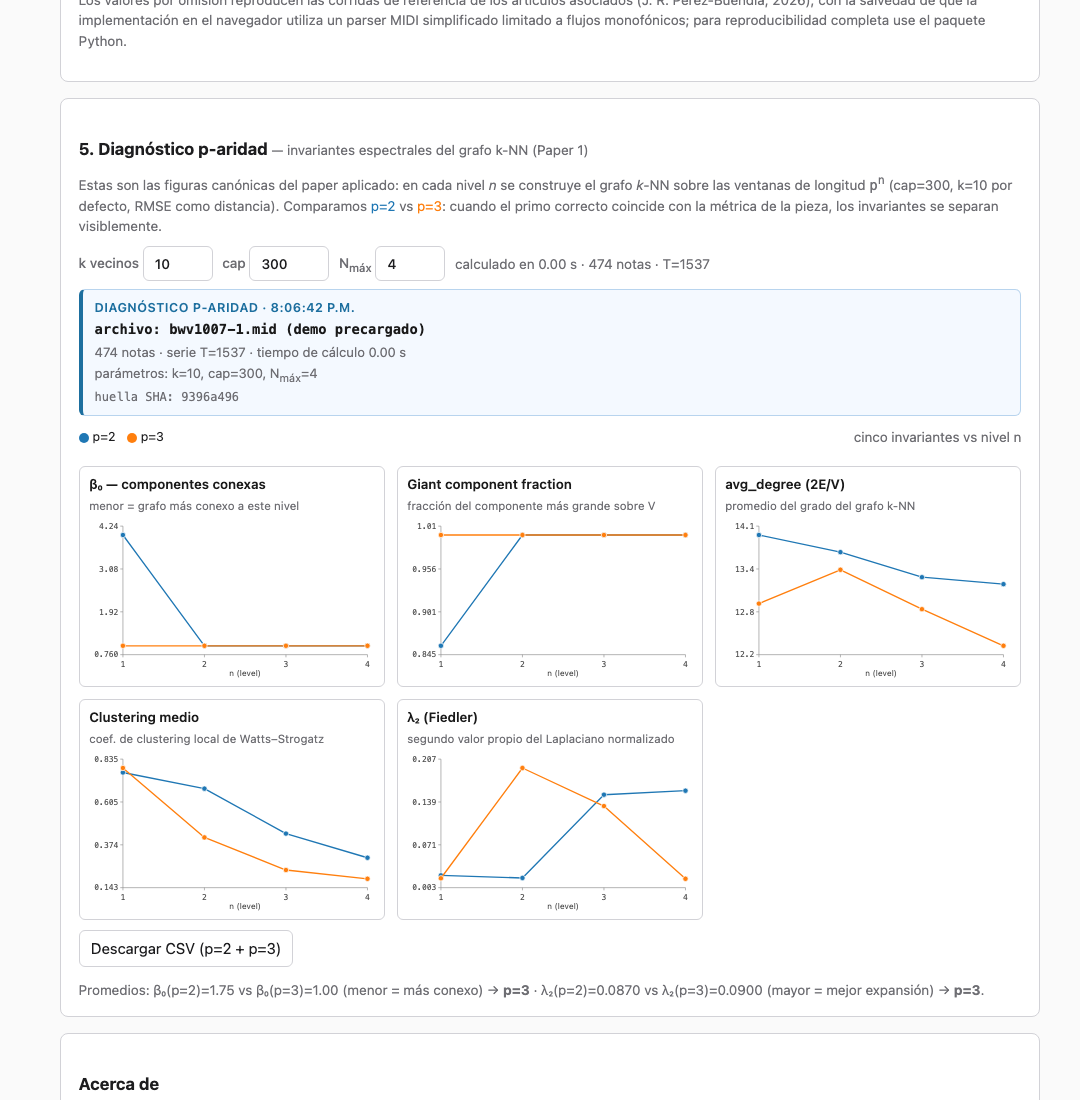
\includegraphics[width=0.97\textwidth]{figs/applet_panel5_diag.png}
  \caption{Sección~5 del applet (versión española, demo BWV~1007).
  De izquierda a derecha y arriba a abajo:
  $\beta_0$, fracción del componente gigante, grado promedio,
  \emph{clustering} medio y $\lambda_2$ de Fiedler vs nivel~$n$,
  comparando $p=2$ (azul) y $p=3$ (naranja). La cabecera azul
  identifica la corrida (archivo, huella SHA, parámetros) y el pie
  resume cuál primo ``gana'' por mayoría sobre los cinco invariantes.
  Para BWV~1007 la torre se vuelve totalmente conexa desde el nivel
  $n=2$ con ambos primos: el invariante actúa como
  \emph{diagnóstico de robustez}, no como certificación automática
  de aridad.}
  \label{fig:applet-panel5}
\end{figure}

La validación numérica de la implementación JavaScript se realizó
contra \code{run\_tower\_on\_beats} ejecutado sobre BWV~1007 con los
mismos hiperparámetros: el número de vértices $V$ coincide
exactamente, las aristas $E$ difieren en ${\le}\,1\%$ por empates de
distancia, $\bar{d}$ en ${\le}\,0{,}5$, $\beta_0$ es exacto excepto
en un único nivel donde difiere por uno, y la fracción del componente
gigante coincide con tolerancia ${\le}\,0{,}07$. Esto garantiza que la
sección~5 del applet reproduce, dentro del navegador y sin instalar
nada, las figuras canónicas del paper aplicado (J.~R.~Pérez-Buendía,
2026, \emph{Profinite hierarchical patterns and prime-indexed
multiscale graph diagnostics}).

\subsection{Garantías de privacidad}

El applet es \textbf{cero red}: no realiza peticiones HTTP de ningún
tipo, no carga recursos externos, no usa cookies, no usa
\code{localStorage}, no genera telemetría. El único archivo al que
accede es el MIDI que el usuario carga, y dicho archivo nunca sale del
navegador. Esta propiedad es relevante tanto para la privacidad del
usuario como para la portabilidad: el applet funciona sin conexión a
Internet, lo cual lo hace apropiado para demostraciones en aulas, en
trámites administrativos como el actual, o en entornos con red
restringida.

\subsection{Limitaciones respecto al paquete Python}

\begin{itemize}[noitemsep]
  \item Sólo se exponen los primos $p \in \{2, 3\}$.
  \item El eje en segundos no está implementado (sólo eje en pulsos).
  \item El generador pseudoaleatorio del $k$-medias usa
        \emph{Mulberry32}, mientras que el paquete Python usa
        \emph{PCG64} de NumPy --- los valores pueden diferir en el
        quinto decimal en piezas no canónicas. Los pisos estructurales
        (por ejemplo $\Cohpi(2,n) = 0.500$ exacto en BWV~1007) se
        reproducen exactamente.
\end{itemize}

% ============== 6. Reproducibilidad ==============
\section{Reproducibilidad y validación}\label{sec:repro}

\subsection{Suite de tests}

El paquete incluye 28 tests organizados en cuatro niveles:

\begin{tabularx}{\linewidth}{lXr}
  \toprule
  \textbf{Nivel} & \textbf{Propósito} & \textbf{\# tests} \\
  \midrule
  \code{tests/smoke/}        & Importación de módulos              & 6 \\
  \code{tests/unit/}         & Funciones puras (residuos, distancia, $k$-medias, croma) & 16 \\
  \code{tests/regression/}   & CSV byte-equivalentes contra \code{results/verified/} & 3 \\
  \code{tests/paper\_values/}& Reproducción de valores publicados  & 3 \\
  \midrule
  \textbf{Total} &  & \textbf{28} \\
  \bottomrule
\end{tabularx}

Los tests \code{paper\_values/} verifican explícitamente las
afirmaciones numéricas de los manuscritos asociados:

\begin{itemize}[noitemsep]
  \item \code{test\_floor\_p2\_bwv1007.py} ---
        $\Cohpi(2,n) = 0.500$ exacto para todo $n \geq 1$ en BWV~1007.
  \item \code{test\_sarabande\_p3\_n3.py} ---
        $\Cohpi(3,3) = 0.901$ en la Sarabanda de BWV~1007 (eje
        de pulsos).
  \item \code{test\_prelude\_p3\_mismatched.py} ---
        $\Cohpi(3,n) = 0.358$ en el preludio BWV~1007 cuando $r \neq p$
        (ilustra el Corolario~\ref{cor:aridity}).
\end{itemize}

\subsection{Scripts de orquestación}

\begin{tabularx}{\linewidth}{lX}
  \toprule
  \textbf{Script} & \textbf{Acción} \\
  \midrule
  \code{scripts/reproduce.sh} & Re-corre el pipeline canónico desde cero \\
  \code{scripts/validate.sh}  & Verifica los hashes SHA-256 de los CSV producidos \\
  \code{scripts/snapshot\_version.sh} & Genera el ZIP de fuentes y su hash \\
  \code{scripts/make\_indautor\_dossier.sh} & Ensambla el dossier INDAUTOR \\
  \bottomrule
\end{tabularx}

\subsection{Resultado de la última ejecución}

A la fecha de cierre de esta versión (\textbf{2026-04-29}), la suite de
tests reporta:

\begin{lstlisting}[style=plain]
============================== test session starts ===============================
platform darwin -- Python 3.13.3, pytest-9.0.3, pluggy-1.6.0
collected 28 items

tests/paper_values/test_floor_p2_bwv1007.py       PASSED
tests/paper_values/test_prelude_p3_mismatched.py  PASSED
tests/paper_values/test_sarabande_p3_n3.py        PASSED
tests/regression/...                               PASSED
tests/smoke/...                                    PASSED
tests/unit/...                                     PASSED

============================== 28 passed in 1.03s ================================
\end{lstlisting}

% ============== 7. Registro INDAUTOR ==============
\section{Registro autoral en INDAUTOR}\label{sec:indautor}

\subsection{Datos del solicitante (autor)}

\begin{tabularx}{\linewidth}{lX}
  \toprule
  Nombre completo (legal) & Jesús Rogelio Pérez Buendía \\
  Firma de publicación    & J. Rogelio Pérez-Buendía \\
  Nacionalidad            & Mexicana \\
  Fecha de nacimiento     & 06 de diciembre de 1976 \\
  RFC                     & PEBJ761206N72 \\
  CURP                    & PEBJ761206HDFRNS11 \\
  ORCID                   & \href{https://orcid.org/0000-0002-7739-4779}{0000-0002-7739-4779} \\
  Página web institucional& \url{https://www.cimat.mx/~rogelio.perez} \\
  Página de alojamiento del software & \url{http://personal.cimat.mx:8181/~rogelio.perez/desarrollo-tecnologico/} \\
  Domicilio para notificaciones & CIMAT-Mérida, Carr.\ Sierra Papacal--Chuburná Pto.\ Km 5, C.P. 97302, Mérida, Yuc. \\
  Teléfono                & 55 32 29 35 21 \\
  Correo electrónico      & \href{mailto:rogelio@cimat.mx}{rogelio@cimat.mx} \\
  \bottomrule
\end{tabularx}

\subsection{Datos de la obra}

\begin{tabularx}{\linewidth}{lX}
  \toprule
  Tipo de obra & Programa de Computación (art.\ 13 fr.\ XI LFDA) \\
  Título completo & PAdicMIDI --- A Python Toolkit for Hierarchical, Ultrametric, and $p$-adic Analysis of Symbolic Music Data \\
  Versión & 1.0.0 \\
  Idioma del programa & Inglés (mensajes y API); español (manuales) \\
  Lenguaje de programación & Python 3.10+ \\
  Sistema operativo & macOS, Linux, Windows \\
  Lugar de creación & Mérida, Yucatán, México \\
  Fecha de primera fijación & 2026-02-06 \\
  Fecha de la versión registrada & 2026-04-29 \\
  Carácter de la titularidad & Titular originario (autor único) \\
  Licencia del código fuente & MIT (texto íntegro en \code{LICENSE}) \\
  Licencia de la documentación & CC-BY 4.0 \\
  \bottomrule
\end{tabularx}

\subsection{Identificación criptográfica del paquete}

\begin{tabularx}{\linewidth}{lX}
  \toprule
  Archivo de fuentes & \code{indautor/padicmidi-v1.0.0-source.zip} \\
  Tamaño             & 508\,372 bytes ($\approx$ 496 KB) \\
  SHA-256            & \texttt{\detokenize{cbfb8bab6b9a03d086d0a9463668572d150e5ee7bfd1c93a6ba83d89c44e3ef3}} \\
  \bottomrule
\end{tabularx}

\medskip

El manifiesto completo de archivos individuales con sus hashes SHA-256
se encuentra en el apéndice~\ref{app:manifest}.

\subsection{Declaración bajo protesta de decir verdad}

El suscrito declara que la obra cuyo registro se solicita es de su
autoría original e individual; que no se han incluido fragmentos de
obra de terceros sin la debida atribución, las cuales constan en el
archivo \code{CONTRIBUTION-STATEMENT.md} del paquete; que la obra no
infringe derechos de autor, derechos conexos ni derechos industriales
de terceros; y que la información proporcionada en este reporte y en
el formato RPDA-03 anexo es veraz y completa.

\bigskip
\bigskip
\bigskip

\noindent
\rule{6cm}{0.4pt}

\textbf{Jesús Rogelio Pérez Buendía}\\
{\itshape (firma de publicación: J.~Rogelio Pérez-Buendía)}\\
Mérida, Yucatán, México --- 29 de abril de 2026.

\newpage

% ============== APÉNDICES ==============
\appendix

\section{Listado completo del código fuente}\label{app:source}

Esta sección reproduce íntegramente, en orden topológico de
dependencias, el código fuente Python que conforma la versión 1.0.0 de
PAdicMIDI. Los archivos auxiliares de configuración
(\code{pyproject.toml}, \code{requirements-pinned.txt},
\code{LICENSE}) se incluyen al final del apéndice.

\subsection{API pública del paquete}

\subsubsection{\code{src/padicmidi/\_\_init\_\_.py}}
\lstinputlisting[style=python]{../src/padicmidi/__init__.py}

\subsection{Núcleo numérico (\code{core/})}

\subsubsection{\code{src/padicmidi/core/config.py}}
\lstinputlisting[style=python]{../src/padicmidi/core/config.py}

\subsubsection{\code{src/padicmidi/core/echo.py}}
\lstinputlisting[style=python]{../src/padicmidi/core/echo.py}

\subsubsection{\code{src/padicmidi/core/hierarchical.py}}
\lstinputlisting[style=python]{../src/padicmidi/core/hierarchical.py}

\subsection{Adaptadores de entrada/salida (\code{io/})}

\subsubsection{\code{src/padicmidi/io/midi\_mido.py}}
\lstinputlisting[style=python]{../src/padicmidi/io/midi_mido.py}

\subsubsection{\code{src/padicmidi/io/midi\_pretty.py}}
\lstinputlisting[style=python]{../src/padicmidi/io/midi_pretty.py}

\subsection{Análisis y modelos nulos (\code{analysis/})}

\subsubsection{\code{src/padicmidi/analysis/null\_model.py}}
\lstinputlisting[style=python]{../src/padicmidi/analysis/null_model.py}

\subsubsection{\code{src/padicmidi/analysis/audit.py}}
\lstinputlisting[style=python]{../src/padicmidi/analysis/audit.py}

\subsubsection{\code{src/padicmidi/analysis/aggregate.py}}
\lstinputlisting[style=python]{../src/padicmidi/analysis/aggregate.py}

\subsubsection{\code{src/padicmidi/analysis/directionality.py}}
\lstinputlisting[style=python]{../src/padicmidi/analysis/directionality.py}

\subsection{Ejecutables de línea de comandos (\code{cli/})}

\subsubsection{\code{src/padicmidi/cli/main.py} --- ejecutable unificado}
\lstinputlisting[style=python]{../src/padicmidi/cli/main.py}

\subsubsection{\code{src/padicmidi/cli/run\_one.py}}
\lstinputlisting[style=python]{../src/padicmidi/cli/run_one.py}

\subsubsection{\code{src/padicmidi/cli/run\_suite.py}}
\lstinputlisting[style=python]{../src/padicmidi/cli/run_suite.py}

\subsubsection{\code{src/padicmidi/cli/benchmark.py}}
\lstinputlisting[style=python]{../src/padicmidi/cli/benchmark.py}

\subsubsection{\code{src/padicmidi/cli/job\_list.py}}
\lstinputlisting[style=python]{../src/padicmidi/cli/job_list.py}

\subsubsection{\code{src/padicmidi/cli/mutopia.py}}
\lstinputlisting[style=python]{../src/padicmidi/cli/mutopia.py}

\subsection{Configuración del paquete}

\subsubsection{\code{pyproject.toml}}
\lstinputlisting[style=plain]{../pyproject.toml}

\subsubsection{\code{requirements-pinned.txt}}
\lstinputlisting[style=plain]{../requirements-pinned.txt}

\subsubsection{\code{LICENSE} (MIT)}
\lstinputlisting[style=plain]{../LICENSE}

\section{Manifiesto SHA-256 del dossier}\label{app:manifest}

El siguiente manifiesto enumera todos los archivos del dossier INDAUTOR
con su hash SHA-256 individual. Cualquier modificación posterior de
cualquiera de estos archivos invalidaría el hash global del ZIP de
fuentes. El manifiesto se regenera automáticamente con el script
\code{scripts/make\_indautor\_dossier.sh}.

\lstinputlisting[style=plain]{../indautor/manifiesto-archivos.md}

\section{Cómo subir el software a la página personal}\label{app:upload}

El paquete está preparado para ser publicado en
\url{http://personal.cimat.mx:8181/~rogelio.perez/desarrollo-tecnologico/}
(URL canónica futura: \url{https://www.cimat.mx/~rogelio.perez/desarrollo-tecnologico/}).
La carpeta \code{web-site/} contiene exactamente cuatro archivos HTML
autocontenidos listos para subir tal cual:

\begin{lstlisting}[style=plain]
web-site/
├── index.html       Landing en español (página principal)
├── index.en.html    Landing en inglés
├── applet.html      Applet de análisis (inglés)
└── applet-es.html   Applet de análisis (español)
\end{lstlisting}

\paragraph{Vía SSH / SCP.}

\begin{lstlisting}[style=shell]
# Subir los cuatro archivos HTML al servidor:
scp web-site/*.html rogelio@personal.cimat.mx:~/public_html/desarrollo-tecnologico/padicmidi/

# O bien por rsync:
rsync -av web-site/ rogelio@personal.cimat.mx:~/public_html/desarrollo-tecnologico/padicmidi/
\end{lstlisting}

\paragraph{Vía sitio Hugo (Hugo Blox).} Si la página personal del autor
está construida con Hugo, copiar los applets a \code{static/}:

\begin{lstlisting}[style=shell]
cp web-demo/applet.html web-demo/applet-es.html \
   ~/sitio-hugo/static/desarrollo-tecnologico/padicmidi/
\end{lstlisting}

y enlazar desde la página de \emph{Desarrollo de software} con un
\code{<iframe>} o un botón \emph{``Abrir la demo web''}, en línea con
el patrón ya empleado para \emph{p-adic GRN Suite}.

\paragraph{Aviso legal sugerido para la página de descarga.}

\begin{quote}\itshape
\textbf{Derechos de autor (obra software).} \copyright\ 2026
Jesús Rogelio Pérez Buendía. Derechos de autor en trámite ante el
INDAUTOR (formato RPDA-03), con base en los artículos 13 fracción XI y
24 a 26 de la Ley Federal del Derecho de Autor. El código fuente se
distribuye bajo \emph{licencia MIT}; la documentación y los resultados
verificados, bajo \emph{Creative Commons Attribution 4.0 Internacional}
(CC-BY 4.0). Se reservan los derechos morales reconocidos por los
artículos 18 a 23 de la LFDA.
\end{quote}

\section{Resumen de archivos del dossier INDAUTOR}\label{app:dossier}

\begin{tabularx}{\linewidth}{lX}
  \toprule
  \textbf{Archivo} & \textbf{Contenido} \\
  \midrule
  \code{indautor/RPDA-03-prefilled.md}     & Pre-llenado del formato oficial \\
  \code{indautor/carta-titularidad.md}     & Carta de titularidad firmada \\
  \code{indautor/descripcion-funcional.md} & Descripción funcional ampliada \\
  \code{indautor/VERSION-REGISTRADA.md}    & Identificación de la versión y hash global \\
  \code{indautor/manifiesto-archivos.md}   & Hashes SHA-256 individuales \\
  \code{indautor/manual-usuario.md}        & Manual de usuario (copia) \\
  \code{indautor/manual-tecnico.md}        & Manual técnico (copia) \\
  \code{indautor/codigo-fuente/}           & Copia del paquete \code{src/padicmidi/} \\
  \code{indautor/evidencia-corridas/}      & Logs de tests y quickstart con CSV resultantes \\
  \code{indautor/padicmidi-v1.0.0-source.zip} & Paquete fuente firmado por hash \\
  \code{indautor/REPORTE-TECNICO.pdf}      & Este documento \\
  \bottomrule
\end{tabularx}

\bigskip
\bigskip

\begin{thebibliography}{9}
  \bibitem{paper1}
  Pérez-Buendía, J.~R.,
  \emph{Prime-power indexed multiscale graph diagnostics for symbolic
  temporal data: methodological exploration and delimitation via
  BWV~1007}, sometido a \emph{Journal of Mathematics and Music}
  (Taylor \& Francis), 2026.

  \bibitem{paper2}
  Pérez-Buendía, J.~R.,
  \emph{Profinite hierarchical patterns and prime-indexed multiscale
  invariants in symbolic music}, sometido, 2026.
\end{thebibliography}

\end{document}
